\documentclass[a4paper,11pt]{article}
\usepackage{color}
\usepackage{graphicx}
\usepackage{subcaption}
\usepackage{amsmath}

\graphicspath{ {images/} }
\begin{document}
\title{\color{red}CARNEGIE MELLON UNIVERSITY\\
APPLIED STOCHASTIC PROCESSES  (COURSE 18-751)\\
HOMEWORK 1}
\author{Daniel Fekadu}
\date{\today}
\maketitle
\newpage
\section{prove with Venn diagrams}
\subsection*{(a) $A \cap B^c = A-B$}
\begin{figure}[h]
    \centering
    \begin{subfigure}[b]{0.25\textwidth}
        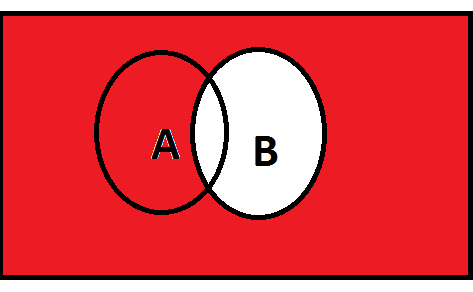
\includegraphics[width=\textwidth]{BC}
        \caption{$B^c$}
    \end{subfigure}
 ~
    \begin{subfigure}[b]{0.25\textwidth}
        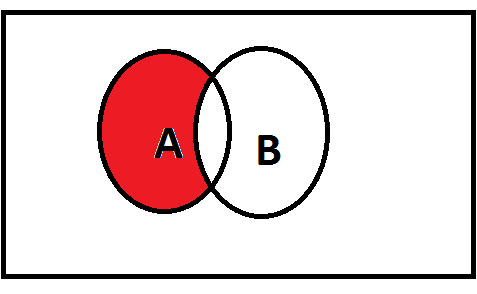
\includegraphics[width=\textwidth]{AnBc}
        \caption{$A \cap B^c$}
    \end{subfigure}
 ~
    \begin{subfigure}[b]{0.25\textwidth}
        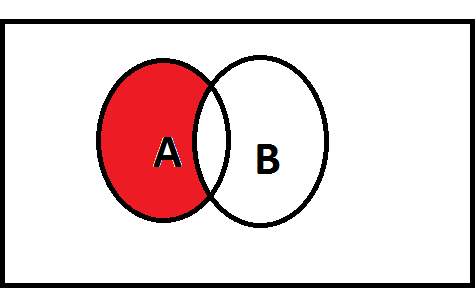
\includegraphics[width=\textwidth]{A-B}
        \caption{$A-B$}
        \label{fig:mouse}
    \end{subfigure}
\end{figure}
this implies $A \cap B^c = A-B$ is true
\subsection*{(b) $A \cup B^c = (A^c\cap B)^c$}
\begin{figure}[hb]
  \centering
    \begin{subfigure}[b]{0.25\textwidth}
        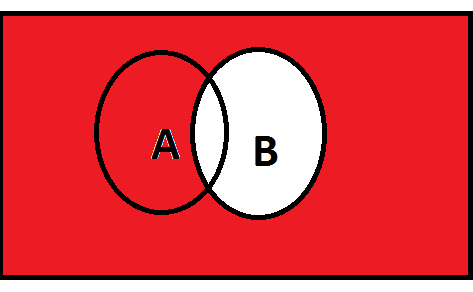
\includegraphics[width=\textwidth]{BC}
        \caption{$B^c$}
    \end{subfigure}
 ~
    \begin{subfigure}[b]{0.25\textwidth}
        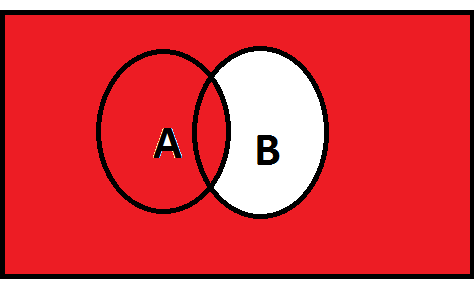
\includegraphics[width=\textwidth]{AuBc}
        \caption{$A \cup B^c$}
    \end{subfigure}
 ~
    \begin{subfigure}[b]{0.25\textwidth}
        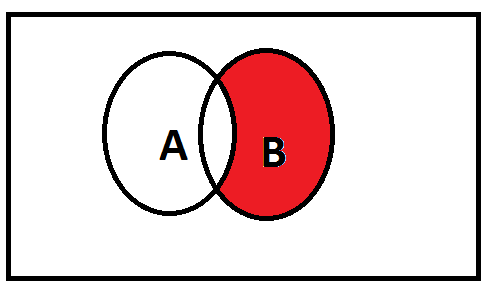
\includegraphics[width=\textwidth]{AcnB}
        \caption{$A^c\cap B$}
        \label{fig:mouse}
    \end{subfigure}
 ~
    \begin{subfigure}[b]{0.25\textwidth}
        \includegraphics[width=\textwidth]{AcnBc}
        \caption{$(A^c \cap B)^c$}
        \label{fig:mouse}
    \end{subfigure}
\end{figure}
this implies $A \cup B^c = (A^c\cap B)^c$ is true
\subsection*{(c) $B-A \neq A-B$}
\begin{figure}[h]
    \centering
    \begin{subfigure}[b]{0.35\textwidth}
        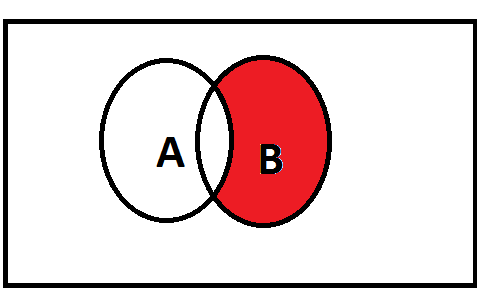
\includegraphics[width=\textwidth]{B-A}
        \caption{$B-A$}
    \end{subfigure}
    \begin{subfigure}[b]{0.35\textwidth}
        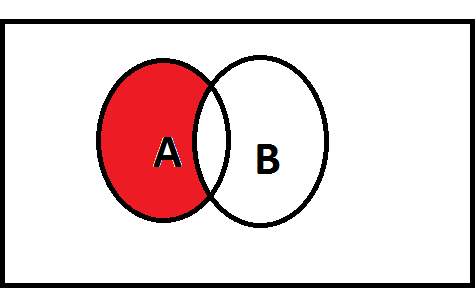
\includegraphics[width=\textwidth]{A-B}
        \caption{$ A-B$}
    \end{subfigure}
\end{figure}
this implies $B-A \neq A-B$ is true
\newpage
\section{}
\subsection*{(a) Irreduciblity and periodicity }
The Markov Chain is irreducible because we can go from any of the states to the other states in finit number of steps
It is also aperiodic[Justfy]
\subsection*{(b) invariant distribution $\pi$ }
\begin{eqnarray}
\pi_j = \sum_{n=0}^{n} \pi_k p_{kj}
\end{eqnarray}•

\begin{eqnarray}
\pi_0 = \pi_0 P_{00} + \pi_1 P_{10} + \pi_2 P_{20}\\
\pi_1 = \pi_0 P_{01} + \pi_1 P_{11} + \pi_2 P_{21}\\
\pi_2 = \pi_0 P_{02} + \pi_1 P_{12} + \pi_2 P_{22}\\
\end{eqnarray}

%i.e $\pi = \pi P$\\

$$
P=\begin{bmatrix} 
0.3 & 0.7 & 0 \\
0.1 & 0.4 & 0.5\\
1    & 0     &0
\end{bmatrix}
$$


\begin{eqnarray}
\pi_0 = 0.3\pi_0+ 0.1\pi_1 + \pi_2 \\
\pi_1 = 0.7\pi_0+ 0.4\pi_1  \\
\pi_2 = 0.5\pi_1\\ 
\pi_0+\pi_1+\pi_2 = 1
\end{eqnarray}•

lets write everything interms of $\pi_0$\\
\begin{eqnarray}
\pi_1=\pi_1\\
\pi_2=0.5\pi_1\\
\pi_0 = 0.3\pi_0+0.1\pi_1+0.5\pi_1\\
0.7\pi_0=0.6\pi_1\\
\pi_0 = \frac{6}{7}\pi_1\\
\pi_0+\pi_1+\pi_2=\frac{6}{7}\pi_1+\pi_1+0.5\pi_1=1
\end{eqnarray}•
\begin{eqnarray}
\frac{33}{14}\pi_1=1\\
\pi_1=\frac{14}{33}\\
\pi_0=\frac{6}{7}.\frac{14}{33}=\frac{4}{11}\\
\pi_2=0.5.\frac{14}{33}=\frac{7}{33}
\end{eqnarray}•
Ans.
$$
\pi = \begin{bmatrix}
\frac{4}{11} \quad \frac{14}{33}\quad \frac{7}{33}   
\end{bmatrix}•
$$

$$
\pi \approx \begin{bmatrix}
0.3636 \quad 0.4242 \quad   0.2121
\end{bmatrix}•
$$
\subsection*{(c) Expected Time from 0 to 2}
$$\beta(2) = 0$$
$$\beta(0) = 1+0.7\beta(1) + 0.3\beta(0)$$
$$\beta(1) = 1+0.1\beta(1) +0.4\beta(1) + 0.5\beta(2) $$
since $\beta(2)=0$
$$\beta(1) = 1+0.1\beta(0) + 0.4\beta(1)$$
$$\beta(0) = 1+0.3\beta(0) + 0.7\beta(1)$$
$$0.7\beta(0)-0.7\beta(1) = 1$$
$$0.6\beta(1)-0.1\beta(0) = 1$$
solving the eqn n1 and n2 we get $\beta(0) = 3.708$ and $\beta(1)= 2.286$
so the expected time from $0$ to $2$ is $ 3.708$


\newpage

\subsection*{(d) Probability that starting from 0, the MC has reached 2 after $n$-steps  vs $ n$}
\begin{figure}[h]
        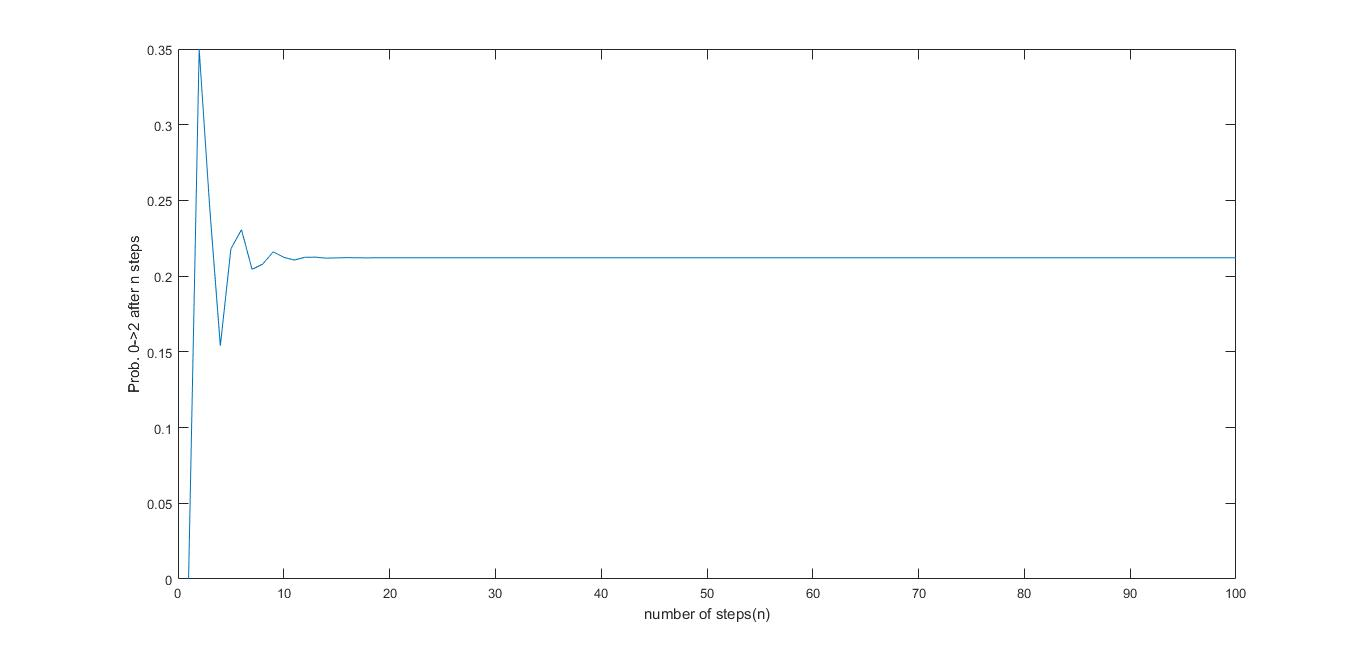
\includegraphics[scale=0.35]{2d}
        \caption{Probability that starting from 0, the MC has reached 2 after $n$-steps  vs $ n$}
\end{figure}
\newpage

\subsection*{(e) Expected Time from 0 to 2}
\begin{figure}[h]
        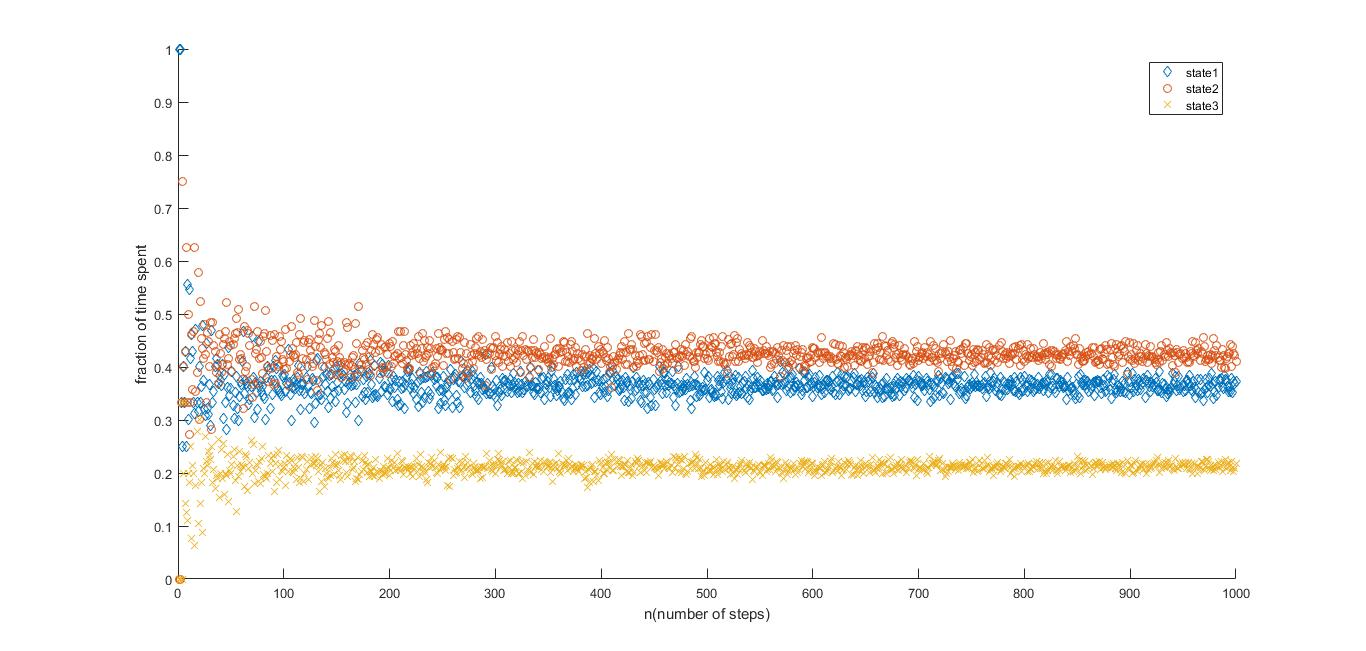
\includegraphics[scale=0.35]{2e}
        \caption{Probability that starting from 0, the MC has reached 2 after $n$-steps  vs $ n$}
\end{figure}
\newpage
\subsection*{(f) $\pi_n$  vs $n$}
\begin{figure}[htbp]
        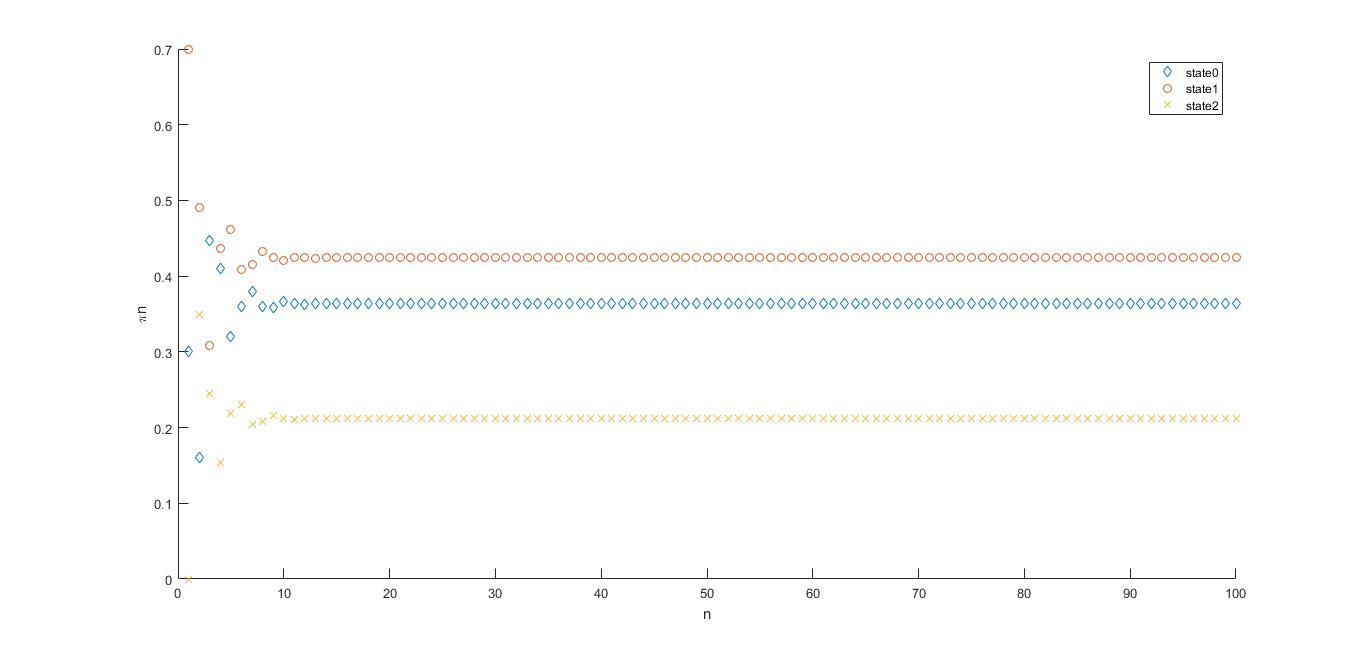
\includegraphics[scale=0.35]{2f}
        \caption{$\pi_n$ vs $n$}
\end{figure}
\newpage 
\section*{Q3}
\end{document}